\documentclass[12pt]{article}
\usepackage{natbib}
\usepackage{hyperref}
\usepackage{graphicx}
\usepackage{subcaption}
\usepackage{amssymb,amsmath,amsthm}
\usepackage{xcolor}
\usepackage{xspace}
\usepackage[nameinlink,capitalize]{cleveref}
\usepackage{cleveref}
\usepackage[margin=1in]{geometry}
\usepackage{lineno}\renewcommand\thelinenumber{\color{gray}\arabic{linenumber}}
\usepackage{pdflscape}
\usepackage{xspace}
\usepackage{array}

\newcolumntype{L}[1]{>{\raggedright\let\newline\\\arraybackslash\hspace{0pt}}m{#1}}
\newcolumntype{C}[1]{>{\centering\let\newline\\\arraybackslash\hspace{0pt}}m{#1}}
\newcolumntype{R}[1]{>{\raggedleft\let\newline\\\arraybackslash\hspace{0pt}}m{#1}}

\newcommand{\comment}{\showcomment}
\newcommand{\showcomment}[3]{\textcolor{#1}{\textbf{[#2: }\textsl{#3}\textbf{]}}}
\newcommand{\nocomment}[3]{}

\newcommand{\ali}[1]{\comment{magenta}{Ali}{#1}}
\newcommand{\bmb}[1]{\comment{red}{BMB}{#1}}
\newcommand{\todo}[1]{\comment{red}{TODO}{#1}}

\theoremstyle{definition} % amsthm only
\newtheorem{proposition}{Proposition}
\newtheorem{theorem}{Theorem}
 
\bibliographystyle{apalike}

\title{Centrality: A Curve-Based Statistical Discription of an Ensemble}
\author{Ali Gharouni, Ben Bolker}
\begin{document}
\maketitle
\linenumbers

% %%%%%%%%%%%%%%%%%%%%%%%%%%%%%%%%%%%%%%%
\section{Introduction}

\cite{juul2021fixed} presented a useful curve-based alternative to the fixed-time statistics of epidemic curve ensembles. 
They cautioned that standard pointwise (fixed-time) averages may not be appropriate to summerize ensembles of epidemic curves. Particularly, they discussed that miscapturing key features of an epidemic such as the peak numbers of infections, the time of the peak, etc. may result in obscuring the forcast process.
While Juul et al.'s implimented their methodology in functional ranking and establishing the 'central set' out of an ensemble, there is a deep existing literature in functional depth and centrality metrics for high dimension data \citep{lopez2009concept,sun2011functional,sun2012exact}. 

The idea of the functional boxplot goes back farther.
It starts with the notion of depth which was first introduced for multivariate data in an attempt to generalize the ideas of order statistics, ranks and medians into higher dimensions (see for e.g., \cite{mahalanobis1936generalized,tukey1975mathematics}).
The notion of depth was extended for functional data by \citep{lopez2009concept}. They introduced the concept of band depth (BD) for ranking-ordering  a sample of functional data from the center outward. This ordeing enables us to define the functional quantiles, centrality or outlyingness of an observation. Further, the classical boxplot for univariate data was extended to the functional boxplot as a visualization tool.

... Juul's method is a special case of *functional depth* (for which fast computational approximations already exist ...). Functional depth is useful because fast and robust. (Why do Juul et al depart from the 'standard' J=2 approach ... ??)

Examples of data depth include the Mahalanobis depth \citep{mahalanobis1936generalized}
\section{Results}

\begin{figure}[h!]
\centering
\begin{subfigure}[t]{.45\textwidth}
\centering
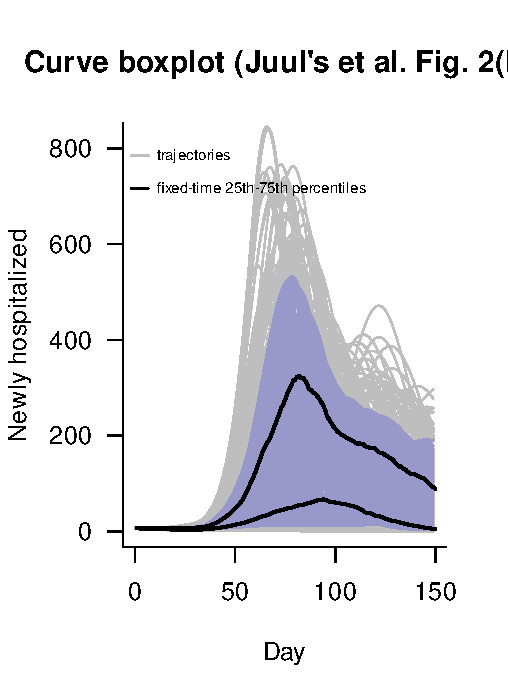
\includegraphics[width=\linewidth]{scripts/pix/fig2b_juul.pdf}
\caption{}\label{p.a}
\end{subfigure}
%
\begin{subfigure}[t]{.45\textwidth}
\centering
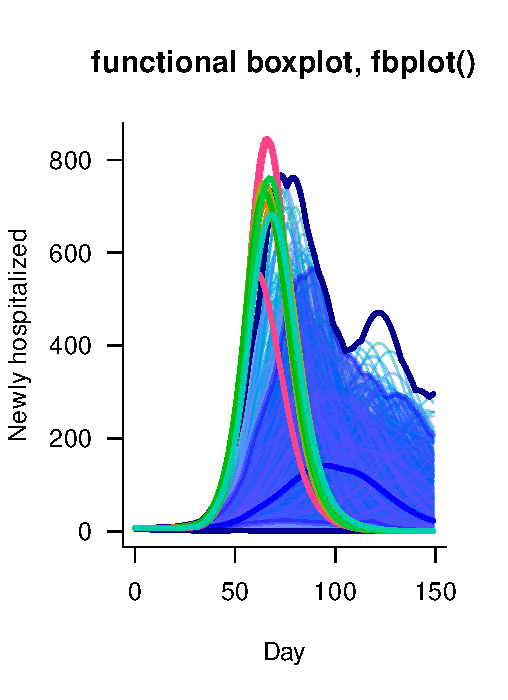
\includegraphics[width=\linewidth]{scripts/pix/fbplot_juul.pdf}
\caption{}\label{p.b}
\end{subfigure}
%
\begin{subfigure}[t]{.45\textwidth}
\centering
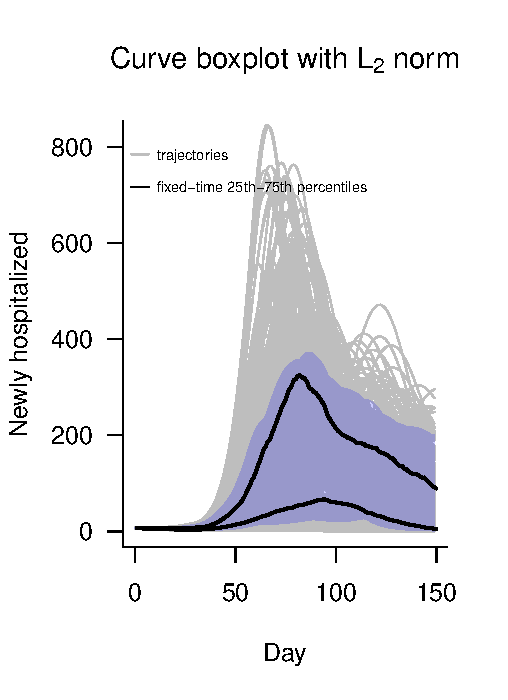
\includegraphics[width=\linewidth]{scripts/pix/L2_juul.pdf}
\caption{}\label{p.c}
\end{subfigure}
%
\begin{subfigure}[t]{.45\textwidth}
\centering
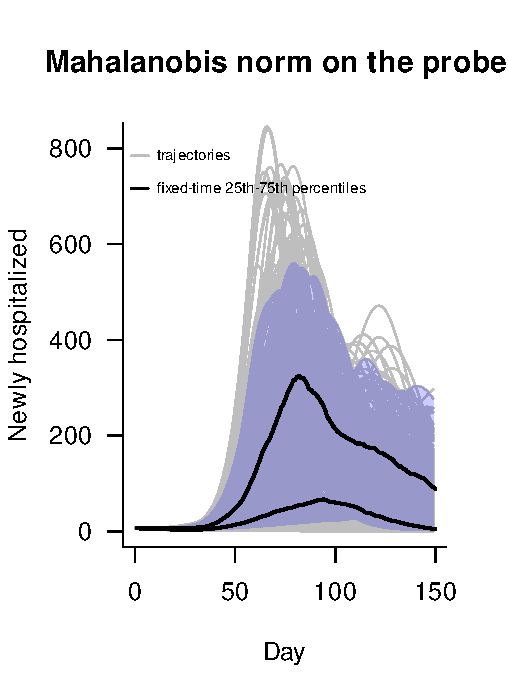
\includegraphics[width=\linewidth]{scripts/pix/mahal_probes_juul.pdf}
\caption{}\label{p.d}
\end{subfigure}
\caption{Other options of curve-based statistics on Juul's et al work}
\label{pan}
\end{figure}


\bibliography{./AliMac}
\end{document}
